\begin{figure}[!t]
  \centering
  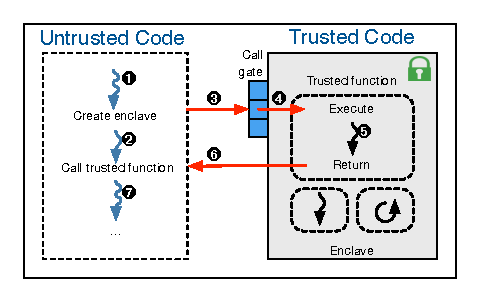
\includegraphics[scale=0.8]{images/sgx.pdf}
  \caption{SGX operating principles.}
  \label{fig:sgx}
\end{figure}

\section{SGX Lightning Tour}
\label{sec:background}
The design of \SYS revolves around the availability of SGX features in the host machines. 
It consists in a form of Trusted Execution Environment (TEE) recently introduced into Intel SkyLake, similar in the spirit to ARM TrustZone~\cite{arm2009security}. 
Applications create secure enclaves to protect the integrity and the confidentiality of the data and the code executed. 
The SGX mechanism, as depicted in Figure~\ref{fig:sgx}, allows applications to access confidential data from inside the enclave. 
The architecture guarantees that an attacker with physical access to a machine won’t be able to tamper with the application data. 
The CPU package represents the security boundary. 
Moreover, data belonging to an enclave is encrypted and authenticated when stored in main memory. 
A memory dump on a victim’s machine will produce encrypted data. 
A remote attestation protocol allows to verify that an enclave run on a genuine Intel processor with SGX. 
An application using enclaves must ship a signed (not encrypted) shared library (\emph{e.g.} a \texttt{.so} in Linux) that can possibly be inspected by malicious attackers. 
The Enclave Page Cache (EPC) is a 128 MB area of memory predefined at boot to store enclaved code and data. 
At most 90 MB can be used by application’s memory pages. 
Any access to an enclave page that dos not reside in the EPC triggers a page fault. 
The SGX driver interacts with the CPU to choose which pages to evict. 
The traffic between the CPU and the system memory is kept confidential by the memory encryption engine (MEE)~\cite{gueron2016memory}, also in charge of tamper resistance and replay protection. 
If a cache miss hits a protected region, the MEE encrypt or decrypt data before sending to, respectively fetching from, the system memory. 
Data can also persisted on stable storage protected by a seal key. 
This is useful in case the application restarts an enclave but without a new remote attestation.

The execution flow of a program using SGX enclaves is like the following.
First, an enclave is created (Figure~\ref{fig:sgx}-\ding{202}).
As soon as a program needs to execute a trusted function (Figure~\ref{fig:sgx}-\ding{203}), it executes SGX's \texttt{ecall} (Figure~\ref{fig:sgx}-\ding{204}).
The call goes through the SGX call gate to bring the execution flow inside the enclave (Figure~\ref{fig:sgx}-\ding{205}).
Once the trusted function is executed by one of the enclave's threads (Figure~\ref{fig:sgx}-\ding{206}), its result is encrypted and sent back the result (Figure~\ref{fig:sgx}-\ding{207}) before giving back the control to the main processing thread (Figure~\ref{fig:sgx}-\ding{208}).